\documentclass[titlepage]{article}
\usepackage{amsmath}
\usepackage{graphicx}

\title{CS 440 - Homework 8}
\author{Matthew Liu - mliu56}
\date{}

\begin{document}
\maketitle{}

Output.txt which holds all output from the program is stored in the zip with the code.\\

\begin{enumerate}
	\item All ss totals (per iteration, per k-itr combination) are reported in output.txt \\
	\item Overall with this data, the higher k is the lower ss total is. At the same time it seems regardless on the cap on iterations, ss total doesn't lower too much, meaning that k-means reaches local optimal solution very fast \\
		\centerline{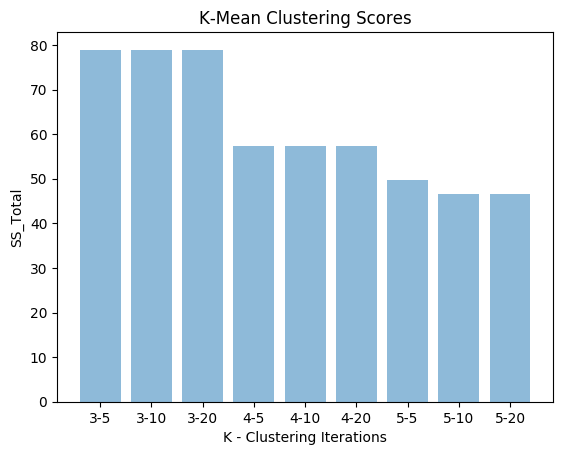
\includegraphics[scale=0.5]{../graph_a.png}}
	\item The reason ss total lowers with higher k is because of the equation of ss total, that is, the sum of all squared distances between each sample and the closest centroid. The higher k is, the more centroids there are, and overall the less samples there are per centroid. Since ss total doesn't average or anything, it directly increases with the amount of samples there are. For this reason, it is not wise to use ss total as a metric for k, as it does not mean anything regarding the accuracy of the clustering \\
	\item Each cluster has the highest percentage of each label calculated, and starting from the highest percentage (regardless of label), that cluster is chosen for that label. The corresponding cluster and label is removed from the list of possibilities, and repeat for the remaining labels. Doing this ensures that the cluster that holds the largest representation per label is chosen for that label. This doesn't defer to ordering of labels, strictly percentage of representation. \\
	\item Individual and Average F1 Scores are reported per k-itr combination in output.txt \\
	\item The Best Average F1 Score and the corresponding centroids for that cluster group are reported in output.txt. As can be seen from the reported individual and average F1 Scores, the best k is 3, as all three iterations (5, 10, 20) reported the same average F1 Score. This makes sense, as even though the more clusters there are (higher k is), the higher precision will be, however on the flip side recall will decrease more than precision will increase as the difference in the number of samples in that cluster becomes too great. Each color represents a cluster, and the triangle shape represents the centroid of that cluster. This best cluster was found by taking the cluster that has the best average F1 score of all combinations of k-itr (and these values can be compared in output.txt)\\
		\centerline{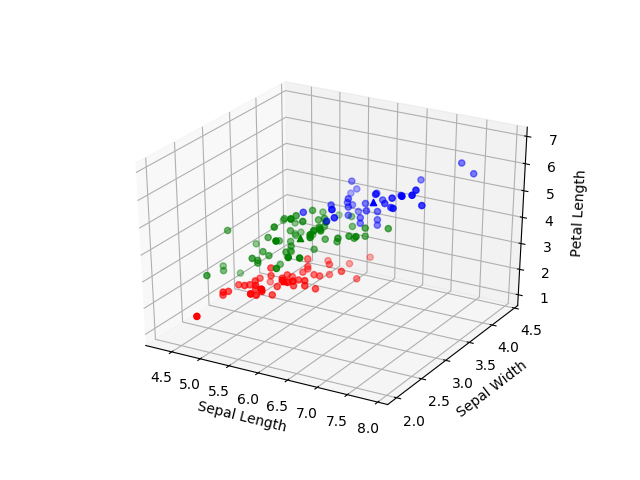
\includegraphics[scale=0.5]{../slswpl.png} 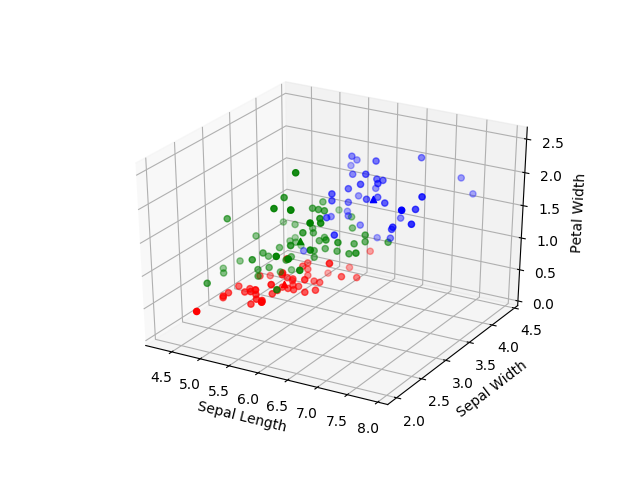
\includegraphics[scale=0.5]{../slswpw.png}}
		\centerline{}
		\centerline{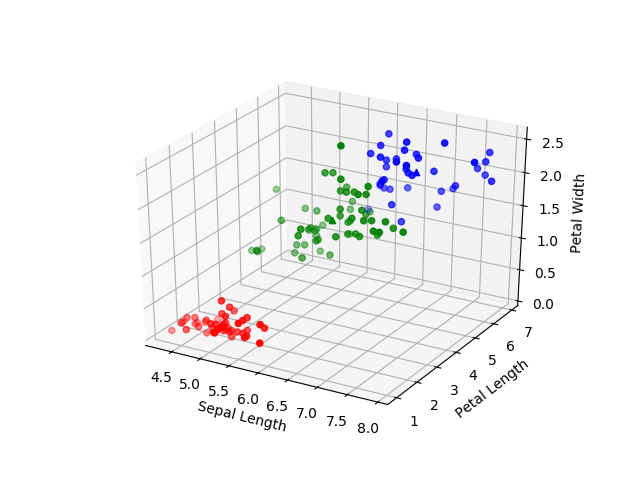
\includegraphics[scale=0.5]{../slplpw.png} 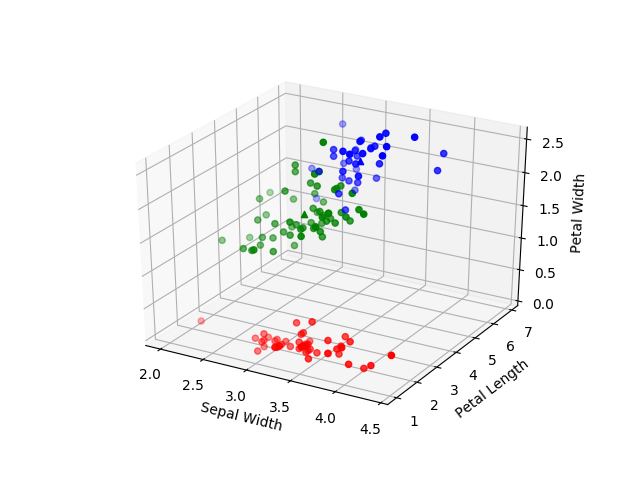
\includegraphics[scale=0.5]{../swplpw.png}}
\end{enumerate}

\end{document}